% !TeX root = ../main-paper.tex
\begin{figure}[!h]
    \centering
    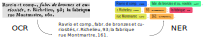
\includegraphics[width=.9\textwidth]{figs/overview-intro.pdf}
    \caption{%
    Overview of the pipeline under study.
    From previously-extracted images of directory entries, 
    we perform OCR and named entity recognition (NER) using different techniques.
    We aim at answering the following questions:
    \emph{How noisy are modern, out-of-the-box OCR systems?}
    \emph{What is the behavior of NER when OCR is noisy?}
    \emph{Can NER be made more robust to OCR noise?}
    }
    \label{<label>}
\end{figure}
\clearpage% force float flush!

\section{Introduction}

% General context + scope limitation
OCRed texts are generally not sufficient to build a high level, semantic view of a collection of historical documents.
A subsequent stage is often needed to extract the pieces of information most likely to be searched for by users, such as named entities: people, organizations, dates, places, etc.
Indeed, being able to properly tag text tokens unlocks the ability to relate entities, and provide colleagues from other fields with databases ready for exploitation.

Being active research topics, OCR and named entity recognition (NER) are still difficult tasks when applied to historical text documents.
OCR approaches used for modern documents are likely to struggle even on printed historical documents due multiple causes related to text readability (low resolution scans, inconsistent printing rules, artifacts, show-through), document complexity (intricate and versatile page layout, use of ancient fonts \& special glyphs) and the variability inherent to the huge diversity of historical sources.
On the other hand, NER approaches developed for modern texts suffer from the time gap between the contemporary entities and the entities mentioned in older texts, and also from the errors introduced into the text by the OCR step.

In this article, we focus on a peculiar category of historical printed books: city trade directories of Paris from the XIX\textsuperscript{th} century (1801 - 1854).
They contain hundred-pages long lists of people, along with their activity and their address, and provide valuable fine-grained knowledge to study the social dynamics of the city over time.
Despite containing roughly the same information, the diversity in layouts, information organization and digitizing quality is challenging both for OCR and NER.

In a recent work to locate potentially polluted urban soils \cite{bell2020automated}, trade directories were leveraged to identify and locate all the gas stations in the city of Providence during the XX\textsuperscript{th} century.
The proposed information extraction pipeline extracts texts with OCR, identifies directories entries and recognizes business type and address within each entry.
In the same way, we aim at producing structured spatio-temporal data from Parisian trade directories.
These directories originate from several publishers, their content is organized following different indexing methods (by name, by activity or by address), printed in various layouts, use different fonts.
We therefore investigate several state-of-the-art OCR and NER approaches to assess their usability on the corpus.

The contributions of this article are the following.
% Contributions
\begin{enumerate*}[(i)]
    \item We review state of the art OCR and NER systems for historical documents (\cref{sec:related-work}).
    \item We introduce a new dataset suitable for OCR and NER evaluation (\cref{sec:dataset}).
    \item We measure the performance of three modern OCR systems on real data (\cref{sec:ocr-xp}).
    \item We evaluate modern NER approaches: their requirements in terms of training data, and the effects of pre-training (\cref{sec:ner-xp1}).
    \item We show that Transformed-based NER can benefit from pre-training and fine-tuning to improve its performance on noisy OCR (\cref{sec:ner-xp2}).
\end{enumerate*}


